\section{Giới thiệu các môi trường sử dụng}
\subsection{ROS(Robot Operating System}
Robotics là một trong những mảng phát triển nhanh nhất trong giới công nghệ. Có thể bạn đã nghe hoặc nhìn thấy những ứng dụng như xe tự lái, robot hình người của Tesla hay Boston Dynamics và bắt đầu muốn tìm hiểu hay phát triển sự nghiệp về Robotics. Nhóm đồ án quyết định sử dụng \textbf{Robot Operating System (ROS)} một trong những nền tảng phát triển robot phổ biến nhất hiện nay.
\subsubsection{ROS là gì?}
Robot Operating System - ROS là một nền tảng mã nguồn mở (open-sourced) cung cấp những thư viện và công cụ để xây dựng các ứng dụng liên quan tới robot. Sau hơn 10 năm phát hành, ROS đã và đang được sử dụng rộng rãi trên toàn thế giới cả trong nghiên cứu lẫn trong công nghiệp.
\subsubsection{Tại sao chọn ROS?}
Trên trang chủ của ROS có dòng chữ "Don’t reinvent the wheel. Create something new and do it faster and better by building on ROS!" nôm na nghĩa là không cần phải mất công làm lại những cái có sẵn, ROS giúp bạn dựng lên những thứ mới nhanh và hiệu quả hơn.
Ưu điểm của ROS:
\begin{itemize}
    \item ROS cung cấp những công cụ chuẩn để giúp việc giao tiếp dễ dàng giữa các tác vụ. Ví dụ, hệ thống của bạn có một camera và một cánh tay robot. Bạn muốn lấy hình ảnh từ camera, xử lý hình ảnh đó và yêu cầu robot gắp vật thể nếu nó xuất hiện ở trong ảnh. Có nhiều cách để thực hiện các bước này, nhưng nếu bạn dùng ROS thì việc truyền nhận thông tin giữa các bước trở nên dễ dàng hơn rất nhiều.
    \item ROS có một cộng đồng user và developer vô cùng lớn mạnh. Như mình đã nói ở phần trước, các công ty và viện nghiên cứu lớn trên thế giới đều đã và đang dùng ROS và nó dần trở thành một nền tảng chuẩn cho việc phát triển robot. Điều này có nghĩa là nếu bạn gặp khó khăn khi làm một dự án với ROS thì nhiều khả năng là bạn chỉ cần google là ra câu trả lời, hoặc bạn có thể hỏi trên những diễn đàn và có nhiều người sẵn sàng giúp bạn.
    \item Có vô vàn nhiều những thư viện sẵn có cho các tác vụ khác nhau. Từ những công nghệ mới trong AI, thị giác máy tính (computer vision), xử lý ngôn ngữ tự nhiên (natural language processing) hay điều khiển (control) v.v., tất cả đều có những phần mềm mới nhất (state-of-the-art) mà bạn có thể trực tiếp tải xuống và sử dụng ngay. Những phần mềm tiên tiến này đa số tới từ những tổ chức, công ty, trường đại học hoặc thậm chí cá nhân mà đang họ dùng ROS trong công việc hay nghiên cứu của họ và cho công khai (open source) code những dự án của mình.
    \item ROS hoàn toàn free và được phép dùng trong sản phẩm thương mại. Đây là lý do vì sao các công ty, tổ chức (kể cả những tập đoàn lớn) rất ưa dùng ROS vì nó dễ dàng thử nghiệm, phát triển và thậm chí thương mại hoá sản phẩm của họ một cách tiết kiệm.
\end{itemize}
Nhược điểm của ROS:
\begin{itemize}
    \item ROS không phù hợp cho những ứng dụng yêu cầu hard real-time (thơi gian thực cứng/tức thì). Hard real-time có nghĩa là hệ thống của bạn phải hoàn thành tác vụ chính xác theo những thời hạn (deadlines) qui định. Chỉ cần lỡ một trong những deadline này thì hệ thống sẽ bị lỗi và có thể gây hậu quả nghiêm trọng. 
    \item ROS phải được chạy trên một cấu hình đủ mạnh để đạt hiệu suất tốt nhất. Để có thể sử dụng ROS thì bạn cần một chiếc máy tính, và tùy vào độ phức tạp của ứng dụng mà có những yêu cầu về cấu hình khác nhau. Đối với những ứng dụng phức tạp, bạn có thể cần phải có một PC với một hoặc nhiều card đồ hoạ, còn nếu ứng dụng đơn giản thì có thể chỉ một chiếc Raspberry Pi (4 - 8 GB RAM) là đủ.
    \item Việc quản lý và bảo trì những gói (package) phần mềm trong ROS vẫn còn nhiều bất cập, đặc biệt là cho những sản phẩm thương mại.
\end{itemize}
\newpage
\subsubsection{ROS2}
Robot Operating System 2 (\textbf{ROS 2}) là một hệ thống phát triển mã nguồn mở phổ biến dành cho robot và các ứng dụng tự động hóa. Được phát triển bởi Open Robotics, ROS 2 là phiên bản tiếp theo của ROS, được thiết kế để cải thiện và mở rộng các tính năng của ROS gốc.

\noindent Để tránh tối đa các nhược điểm của \textbf{ROS} nhóm đồ án quyết định sử dụng \textbf{ROS2} thay vì \textbf{ROS}.
\subsubsection*{Tính năng quan trọng của ROS2}


\begin{itemize}
    \item Kiến trúc phân phối mạnh mẽ cho phép chạy trên nhiều nút và thiết bị khác nhau.
    \item Hỗ trợ đa nền tảng, cho phép phát triển trên nhiều hệ điều hành và kiến trúc khác nhau.
    \item Hỗ trợ nhiều ngôn ngữ lập trình như C++, Python và Java.
    \item Cơ sở dữ liệu trạng thái giúp theo dõi trạng thái của các nút trong hệ thống.
    \item Các giao thức truyền dữ liệu như DDS và \textbf{ROS}  Bridge cho phép giao tiếp dễ dàng giữa \textbf{ROS}  và \textbf{ROS 2}.
\end{itemize}
\subsubsection*{So sánh giữa \textbf{ROS} và \textbf{ROS2}}
\begin{center}
\begin{tabular}{|p{4.5cm}|p{4.5cm}|p{4.5cm}|}
\hline
\textbf{Đặc điểm} & \textbf{ROS} & \textbf{ROS 2} \\
\hline
Phiên bản chính & ROS Kinetic (tháng 5/2016) và ROS Melodic (tháng 5/2018) & ROS 2 (phiên bản chính đầu tiên tháng 5/2017) \\
\hline
Ngôn ngữ lập trình & C++ và Python & C++, Python và hỗ trợ cho nhiều ngôn ngữ khác nhau như Rust, Java, ... \\
\hline
Hỗ trợ hệ điều hành & Chủ yếu cho Ubuntu Linux & Hỗ trợ nhiều hệ điều hành, bao gồm Windows, macOS và Linux. \\
\hline
Khả năng real-time & Hỗ trợ kém & Hỗ trợ real-time thông qua ROS 2 Real-time, đặc biệt trong các ứng dụng yêu cầu khả năng real-time. \\
\hline
Cơ chế truyền thông & ROS Networking & DDS (Data Distribution Service) dựa trên mô hình publish-subscribe. \\
\hline
Kiến trúc & ROS 1 sử dụng mô hình single-process (chạy nhiều node trong một tiến trình). & ROS 2 hỗ trợ mô hình multi-process (mỗi node chạy trong một tiến trình riêng biệt). \\
\hline
Bảo mật & Bảo mật yếu & Cải thiện đáng kể về bảo mật với hỗ trợ cho mã hóa và xác thực. \\
\hline
Độ ổn định và tin cậy & ROS 1 thường gặp vấn đề về độ ổn định trong các ứng dụng lớn và phức tạp. & ROS 2 cải thiện đáng kể về độ tin cậy và ổn định. \\
\hline
Hỗ trợ cho ứng dụng nhúng & Có, nhưng hạn chế & Có hỗ trợ tốt cho các ứng dụng nhúng và hệ thống nhúng. \\
\hline
Cộng đồng và hỗ trợ & Cộng đồng lớn, nhiều gói phần mềm và tài liệu. & Cộng đồng đang phát triển, nhưng còn ít so với ROS 1. \\
\hline
Tương thích ngược với ROS 1 & Không tương thích ngược & Có khả năng tương thích ngược thông qua ROS 1 ROS 2 Interface (ROS 1 Bridge). \\
\hline
\end{tabular}
\end{center}

%%%%%%%%%%%%%%%%%%%%%%%%%%%%%%%%%%%%%%%%%%%%%%%%%%%%%%%%%%%%%%%%%%%%%%%%%%%%%%%%%%%%%%%%%%%%%%%%%%%%%%%%%%%
\subsection{Môi trường mô phỏng \textbf{GAZEBO}}
Gazebo là một công cụ mô phỏng môi trường 3D miễn phí và mã nguồn mở, được sử dụng rộng rãi trong nghiên cứu robot. Gazebo cung cấp khả năng mô phỏng các đối tượng vật lý như robot, cảm biến, môi trường,... giúp người dùng có thể thiết kế, kiểm tra và đánh giá các hệ thống robot trong môi trường giống thực tế trước khi triển khai thực tế.\\
Các tính năng nổi bật của GAZEBO bao gồm:
\begin{itemize}
    \item Hỗ trợ mô phỏng động lực học chính xác, áp dụng luật vật lý thực tế lên các vật thể.
    \item Có thư viện mô hình hóa các loại robot như xe điện, máy bay trực thăng, tàu lượn,...với các bộ cảm biến tiêu chuẩn.
    \item Cho phép tùy chỉnh môi trường mô phỏng với các đối tượng như đường, tòa nhà, cây cối, sông, núi, ánh sáng,..
    \item Hỗ trợ tích hợp với các công cụ như ROS (Robot Operating System) để triển khai trên robot thực tế.
    \item Giao diện thân thiện, cho phép theo dõi trực quan quá trình mô phỏng.
\end{itemize}
Do có những ưu điểm trên, Gazebo đã trở thành công cụ mô phỏng tiêu chuẩn được sử dụng rộng rãi trong nghiên cứu và phát triển robot. Việc sử dụng Gazebo giúp tiết kiệm thời gian và chi phí thử nghiệm, đồng thời nâng cao độ an toàn cho quá trình phát triển sản phẩm.



\subsubsection{Xây dựng môi trường trong GAZEBO}
\subsubsection*{Xây dựng môi trường mô phỏng cho xe tự hành trong GAZEBO}

Để xây dựng môi trường mô phỏng cho xe tự hành, đầu tiên cần thiết kế mô hình 3D của các đối tượng trong môi trường như đường, xe cộ, người, cây,... Sau đó nhập các mô hình 3D này vào Gazebo và bố trí chúng phù hợp để tạo thành bản đồ mô phỏng.

\noindent Tiếp theo, mô hình 3D của xe tự hành cũng được nhập vào và đặt vào vị trí ban đầu trong môi trường. Các plugin cảm biến giả lập như camera, Lidar, GPS,...cũng được lựa chọn và gắn vào mô hình xe.\\

\noindent Cuối cùng, các thông số vật lý của môi trường như lực hấp dẫn, ma sát,...được cài đặt phù hợp để mô phỏng chính xác động lực học của xe tự hành khi vận hành. Như vậy, môi trường Gazebo đã sẵn sàng để chạy thử nghiệm các thuật toán điều khiển và điều hướng cho xe tự hành.\\

\noindent Để xây dụng môi trường trong \textbf{GAZEBO} ta cần có \textbf{MODELS} và \textbf{WORLDS}. Do đó để cấu tạo nên một môi trường mô phỏng cụ thể ta phải xử lý cả \textbf{models} và \textbf{worlds}.\\
\subsubsection{Model Editor (Trình chỉnh sửa mô hình)}

Model Editor là một trong những công cụ quan trọng trong \textbf{GAZEBO}, cho phép người dùng tạo và tùy chỉnh các mô hình 3D một cách dễ dàng. Điều này rất hữu ích khi chúng ta cần tạo các đối tượng mô phỏng riêng biệt hoặc tùy chỉnh các mô hình có sẵn để phù hợp với mục đích của mô phỏng.\\

Để sử dụng Model Editor, chúng ta có thể thực hiện các bước sau:

\begin{enumerate}
    \item Mở Model Editor từ giao diện \textbf{GAZEBO}.
    \item Sử dụng các công cụ vẽ để tạo các hình học cơ bản như hình hộp, hình trụ, hình cầu, hoặc nạp các mô hình 3D có sẵn từ thư viện.
    \item Tùy chỉnh các mô hình bằng cách thay đổi kích thước, màu sắc và các thuộc tính khác.
\end{enumerate}

\noindent Model Editor giúp tạo ra các đối tượng mô phỏng đa dạng và phức tạp, tạo điều kiện thuận lợi cho nghiên cứu và phát triển robot.\\

\noindent Ngoài sử dụng các models có sẵn trong thư viện 
\url{https://app.gazebosim.org/dashboard} ta có thể sử dụng những công cụ render 3d như \textbf{Sketch}, \textbf{Blender},.... để tạo ra những models mình mong muốn. Vì cấu tạo của 1 model rất đơn giản:
\begin{enumerate}
    \item file \textbf{materials} chứa hình ảnh mặt ngoài của models.
    \item file \textbf{meshes} chứa hình ảnh 3D models.
    \item file \textbf{.config } khai báo dưới dạng 1 file XML để định nghĩa 1 models trong \textbf{GAZEBO}.
    \item file \textbf{.sdf } khai báo dưới dạng 1 file XML để  mô tả cụ thể về cấu trúc và hình dáng của một mô hình hoặc đối tượng trong môi trường mô phỏng \textbf{GAZEBO}.
\end{enumerate}

\subsubsection*{Building World (Xây dựng môi trường)}

Building World là một tính năng mạnh mẽ trong Gazebo, cho phép người dùng xây dựng và chỉnh sửa môi trường mô phỏng. Chúng ta có thể tạo ra các đối tượng mô phỏng như đường, tòa nhà, cây cối, đồng cỏ, núi, sông, ánh sáng, và nhiều thứ khác để tạo nên một môi trường mô phỏng động và phong phú.

Để sử dụng Building World, chúng ta có thể tuân theo các bước sau:

\begin{enumerate}
    \item Mở Building World trong giao diện Gazebo.
    \item Kéo và thả các đối tượng từ thư viện vào môi trường mô phỏng.
    \item Tùy chỉnh các đối tượng bằng cách thay đổi vị trí, kích thước, màu sắc và thuộc tính khác.
\end{enumerate}

\noindent Building World giúp tạo ra các môi trường mô phỏng đa dạng và phức tạp, phù hợp cho việc thử nghiệm và kiểm tra hệ thống robot trong các tình huống thực tế.\\

\noindent Như vậy, Model Editor và Building World là những công cụ quan trọng trong Gazebo giúp tạo và tùy chỉnh các mô hình 3D và môi trường mô phỏng, giúp tối ưu hóa quá trình phát triển và thử nghiệm robot và ứng dụng tự hành. 


\subsubsection{Mô phỏng Toán học trong Gazebo}

Trong Gazebo, chúng ta có thể sử dụng các phép tính toán và công thức toán học để điều khiển robot. Ví dụ, để điều khiển một robot di chuyển từ điểm A đến điểm B, chúng ta có thể sử dụng các phép toán đại số tuyến tính và tính toán đường đi tối ưu.

\subsubsection*{Ví dụ 1: Điều khiển Robot di chuyển}

Giả sử chúng ta có một robot di chuyển trên mặt phẳng và muốn nó di chuyển từ vị trí $(x_1, y_1)$ đến $(x_2, y_2)$. Chúng ta có thể sử dụng công thức Euclid để tính toán khoảng cách giữa hai điểm:

\begin{equation}
    d = \sqrt{(x_2 - x_1)^2 + (y_2 - y_1)^2}
\end{equation}

Sau đó, chúng ta có thể sử dụng các phép toán vector để tính toán hướng và vận tốc cần thiết để di chuyển robot đến điểm đích.

\subsubsection*{Ví dụ 2: Tính toán Tọa độ Góc}

Để quay robot đến một góc xác định, chúng ta có thể sử dụng các công thức toán học để tính toán tọa độ góc. Ví dụ, để quay robot một góc $\theta$ so với hướng ban đầu, chúng ta có thể sử dụng các phép toán trigonometri như sin và cos để tính toán tọa độ mới $(x', y')$.

\begin{align}
    x' &= x \cos(\theta) - y \sin(\theta) \\
    y' &= x \sin(\theta) + y \cos(\theta)
\end{align}

\subsubsection{Mô phỏng Động lực học trong Gazebo}

Gazebo cho phép chúng ta mô phỏng động lực học của robot và các đối tượng trong môi trường 3D. Chúng ta có thể sử dụng các công thức vật lý và toán học để tính toán hành vi của robot trong các tình huống phức tạp.

\subsubsection*{Ví dụ 3: Mô phỏng Rơi tự do}

Để mô phỏng rơi tự do của một đối tượng, chúng ta có thể sử dụng phương trình của vật lý:

\begin{equation}
    h(t) = \frac{1}{2} g t^2
\end{equation}

Trong đó $h(t)$ là độ cao tại thời điểm $t$, $g$ là gia tốc của trọng trường.

\subsubsection*{Ví dụ 4: Mô phỏng Lực va chạm}

Khi một robot va chạm vào một vật thể, chúng ta có thể sử dụng phương trình Newton để tính toán lực va chạm:

\begin{equation}
    F = ma
\end{equation}

Trong đó $F$ là lực va chạm, $m$ là khối lượng của robot và vật thể, $a$ là gia tốc va chạm.

\subsubsection{Kết Luận }

Toán học đóng vai trò quan trọng trong việc điều khiển, tính toán và mô phỏng robot và môi trường trong Gazebo. Báo cáo này đã trình bày một số ví dụ cụ thể về cách sử dụng toán học trong Gazebo để điều khiển robot và mô phỏng các tình huống phức tạp. Việc hiểu và áp dụng toán học có thể giúp cải thiện khả năng mô phỏng và điều khiển trong nghiên cứu và phát triển robot.\\
\noindent Sử dụng Gazebo trong mô phỏng xe tự hành là một công cụ quan trọng giúp phát triển và kiểm tra các hệ thống xe tự hành. Gazebo cho phép mô phỏng động lực học với độ chính xác cao, áp dụng các luật vật lý thực tế cho các đối tượng trong môi trường mô phỏng. Điều này giúp nhà phát triển kiểm tra và đánh giá hiệu suất của xe tự hành trong các tình huống phức tạp trước khi triển khai trong môi trường thực tế. Gazebo cung cấp thư viện mô hình hóa đa dạng, cho phép tạo ra các môi trường mô phỏng cụ thể với các đối tượng như xe tự hành, cảm biến, và môi trường xung quanh. Sử dụng Gazebo giúp tiết kiệm thời gian và chi phí trong quá trình phát triển và kiểm tra xe tự hành, đồng thời đảm bảo tính chính xác và an toàn của hệ thống.
\subsection{Tạo một số models ứng dụng GAZEBO}
Nhóm có một số models đã mô phỏng được qua \textbf{GAZEBO} mà không cần sử dụng thư viện có sẵn.\\

\begin{figure}[ht]
  \centering
  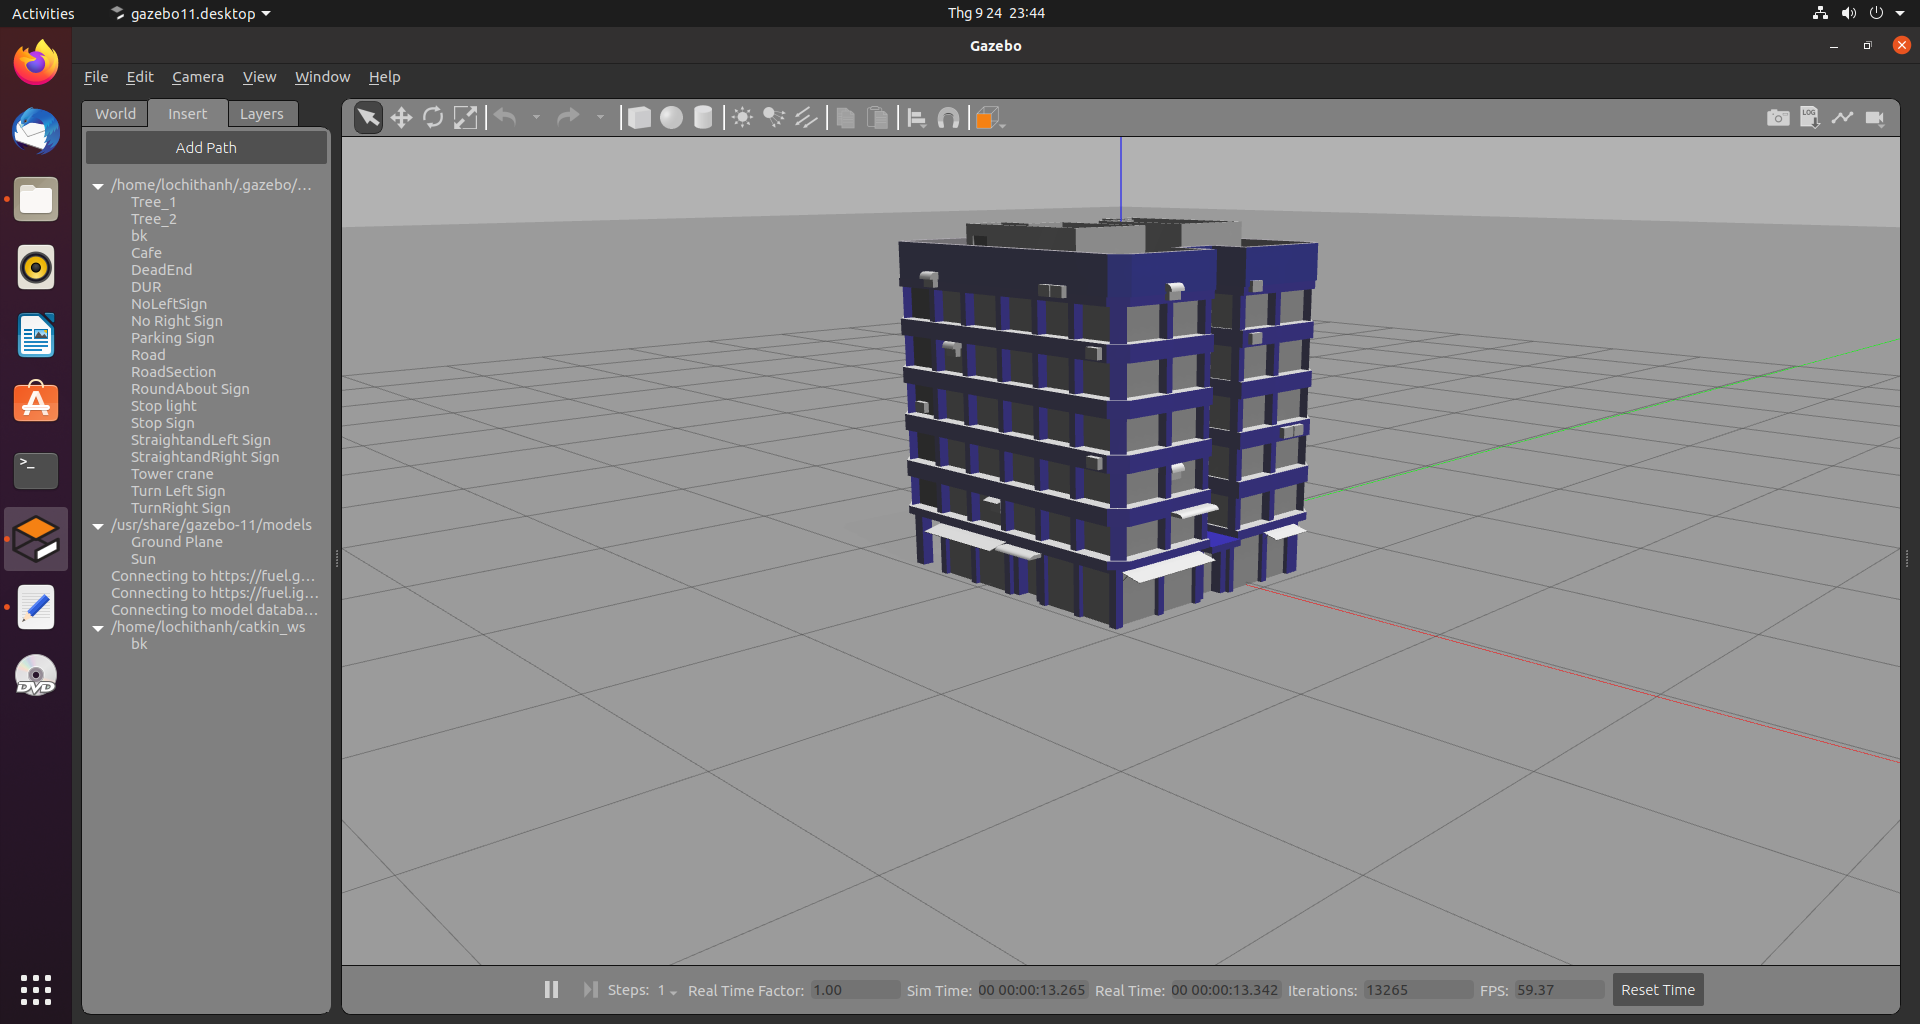
\includegraphics[width=\textwidth]{images/H1.png}
  \caption{Mô hình tòa H3.}

\end{figure}


\begin{figure}[ht]
  \centering
  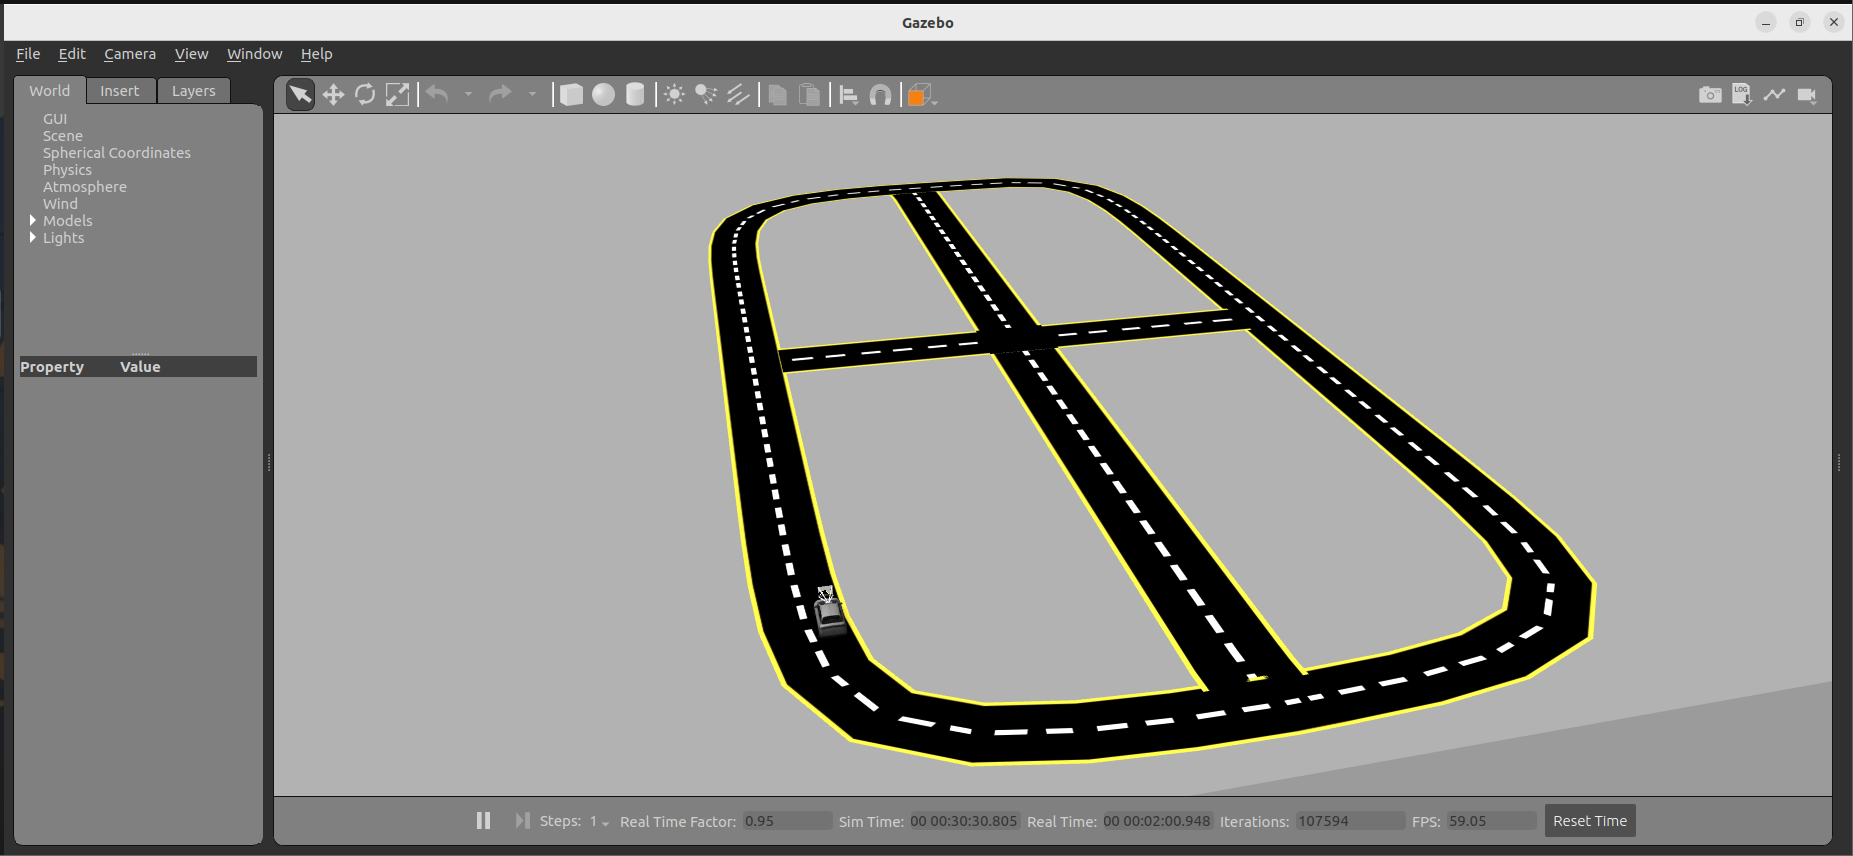
\includegraphics[width=\textwidth]{images/road.png}
  \caption{Test road.}

\end{figure}



















